\documentclass{cernatsnote}
\usepackage[colorinlistoftodos]{todonotes}
\usepackage{placeins}
\usepackage{subcaption}
\usepackage{graphicx}
\usepackage{longtable}
\usepackage{booktabs}
\usepackage{float}

\title{CERN ATS Note title}
\author{
	Author Name \; \\		
	CERN, CH-1211 Geneva, Switzerland
}
\email{tobias.persson@cern.ch}
\date{\today}

\begin{document}
\maketitle

\begin{abstract}

\end{abstract}
\\ \\ \\ 

\begingroup
\color{black}
\tableofcontents
\endgroup

\pagebreak

\section{Introduction}

\section{Local corrections}
\section{Injection}
\subsection{Linear Corrections}
\subsection{Non Linear}
\section{Ramp}
In the beginning of Run~2 the global corrections used at injections were trimmed out linearly from 450~GeV to YYY. This was changed in 2018 because it was observed that the correction was not beneficial in the later stage. The correction was then trimmed out YYYY. This approach was also followed in the 2022 commissioning. In YYY we measured the $\beta$-beat along the ramp using 3 bunches. The use of the 3 bunches was possible due to simulation that considered the machine protection during LS~2\cite{}. In Fig~\ref{fig:ramp_peak_rms} is shown. We notice that there is a peak close to which is a bit higher around 1900~GeV in horizontal and around 3000~GeV in vertical. 

\begin{figure}[ht]
\begin{subfigure}{.5\textwidth}
  \centering
  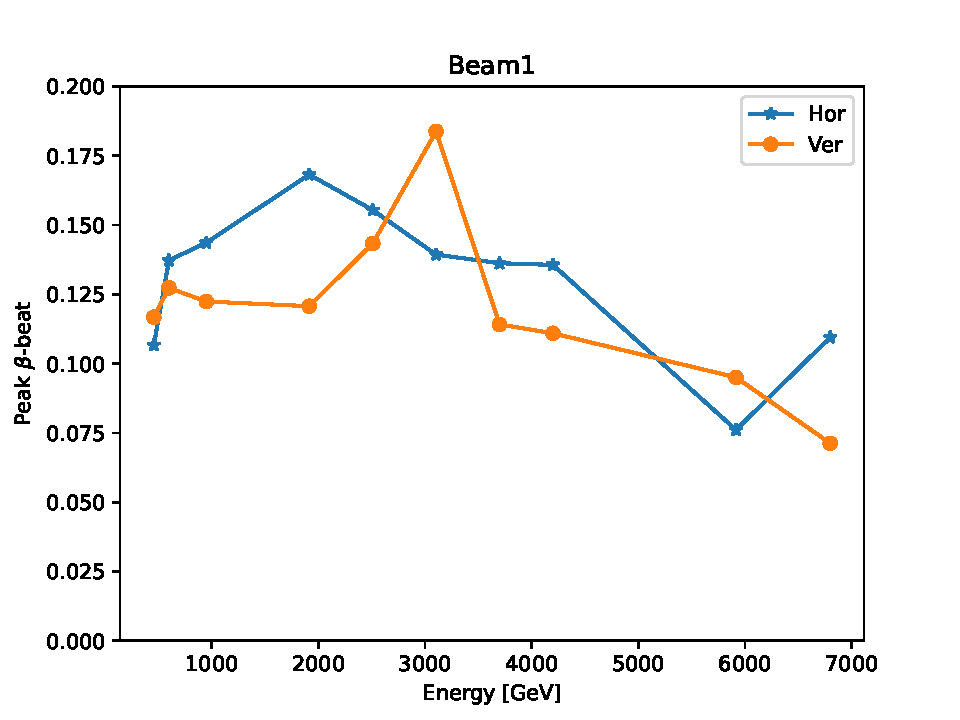
\includegraphics[width=.8\linewidth]{ramp/Beam1_peak_filter.pdf}  
  \caption{Beam~1 peak $\beta$-beat at the different energies during the ramp in 2022.}
\end{subfigure}
\begin{subfigure}{.5\textwidth}
  \centering
  % include second image
  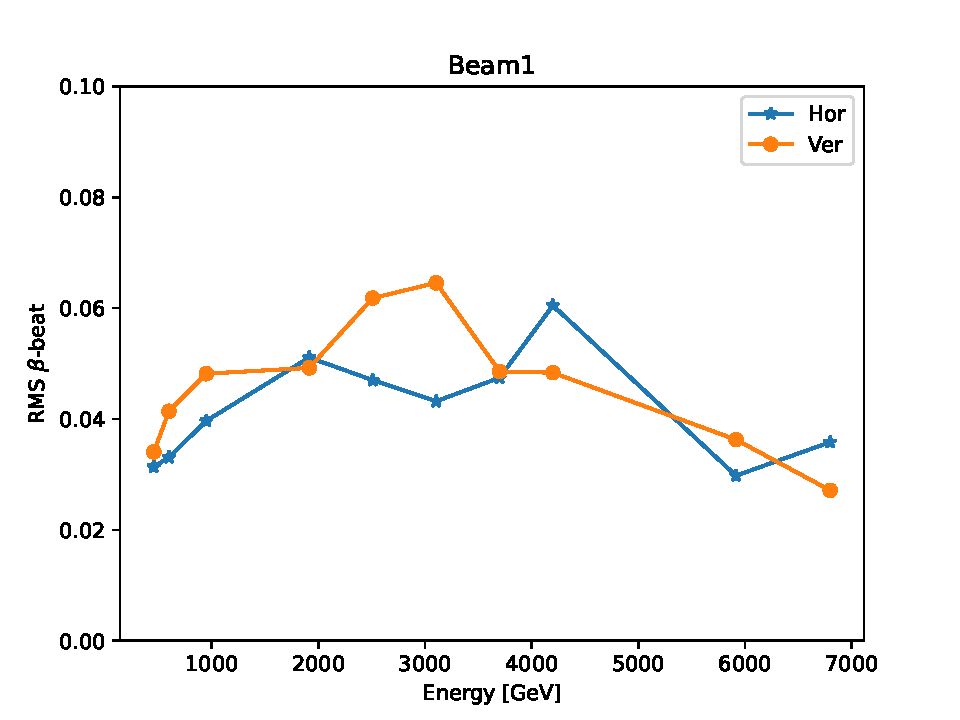
\includegraphics[width=.8\linewidth]{ramp/Beam1_rms_filter.pdf}  
  \caption{Beam~2}
\end{subfigure}
\caption{$\beta$-beat with the LRBB wire On and Off.}
\label{fig:ramp_peak_rms}
\end{figure}

In Fig.~\ref{fig:ramp_mqt} the $\beta$-beat is plotted together with the expected $\beta$-beat from the powering of the MQTs. We can observe that for the peak values they add up in phase with the measured large values. The MQTs are used to correct the tune along the cycle. A difference in how they are operated this year is that the knobs used for tune correction are only utilizing the non-ATS arcs for the corrections. This makes the strength of the magnets stronger which then in turn has a bigger impact on the $\beta$-beat. The $\beta$-beat was still considered to be within a good level and no dedicated correction is needed. However, in view of 2023 it is worth considering of applying a correction.

\begin{figure}[ht]
\begin{subfigure}{.5\textwidth}
  \centering
  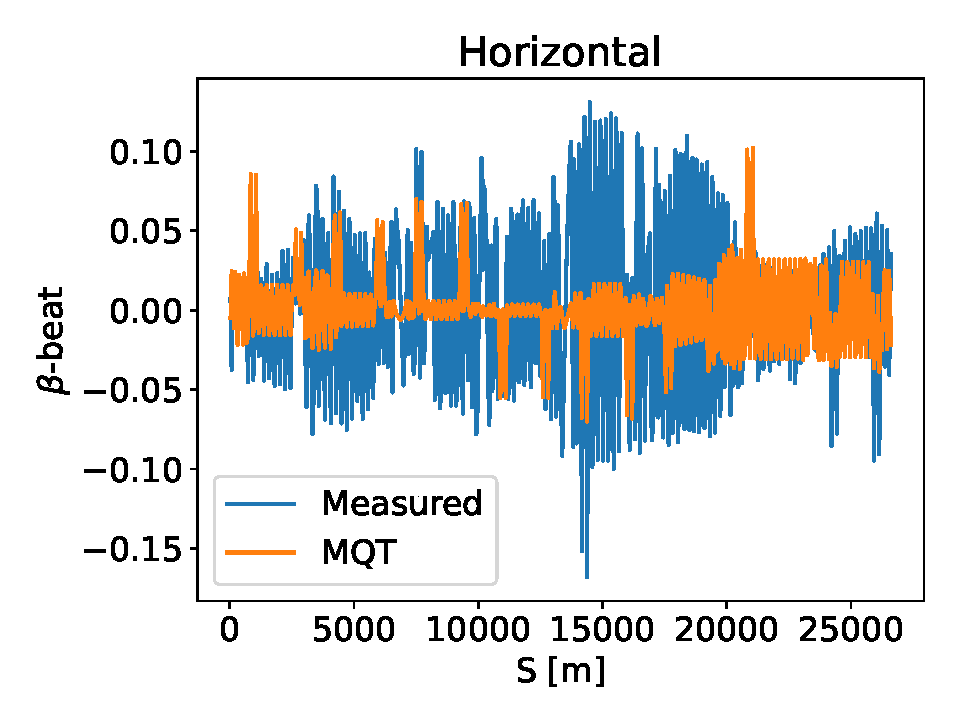
\includegraphics[width=.8\linewidth]{ramp/mqt_in_ramp_1900GeV_horizontal.pdf}  
  \caption{Beam~1 peak $\beta$-beat at the different energies during the ramp in 2022.}
\end{subfigure}
\begin{subfigure}{.5\textwidth}
  \centering
  % include second image
  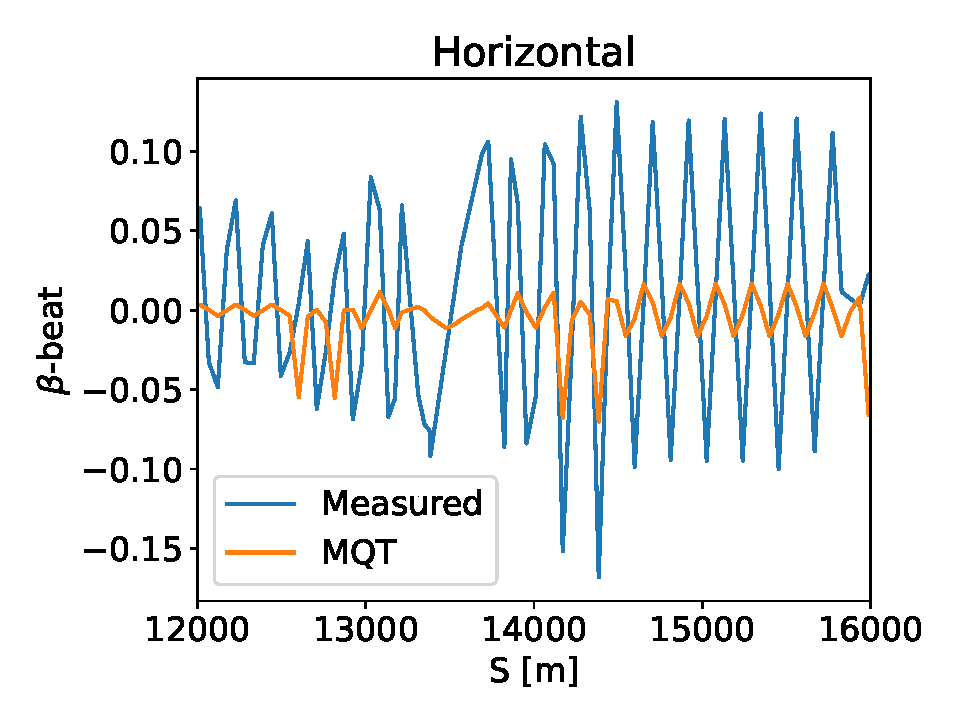
\includegraphics[width=.8\linewidth]{ramp/mqt_in_ramp_1900GeV_horizontal_zoom.pdf}  
  \caption{Beam~2}
\end{subfigure}
\caption{$\beta$-beat with the LRBB wire On and Off.}
\label{fig:ramp_mqt}
\end{figure}

\section{Local}

\section{Wire}
The optics measurements with the LRBB were done on the 4th of August 2022. The powering was done in steps and a sign error was discovered for the compensation part for beam 2. This was quickly solved and after observing that there was no major optics change coming from the wire we did optics measurements both on- and off momentum.

An attempt to do a K-modulation was also performed but the tune signal was too noisy to draw any conclusion. The fact that the tune signal deteriorates when turning on the wire is expected because it creates an octupolar component that deteriotes the tune signal. In case it would be deemed necessary to measure the impact on the $\beta^*$ one should pre-calculate a correction of the MOF and MOD that would cancel the octupolar component of the LRBB-wire. However, from the measurement of the $\beta$-beat using the wire as well as observing the luminoisty when it has been turned on in operation it is possible to conclude that the impact must be very limited. 

\begin{figure}[ht]
\begin{subfigure}{.5\textwidth}
  \centering
  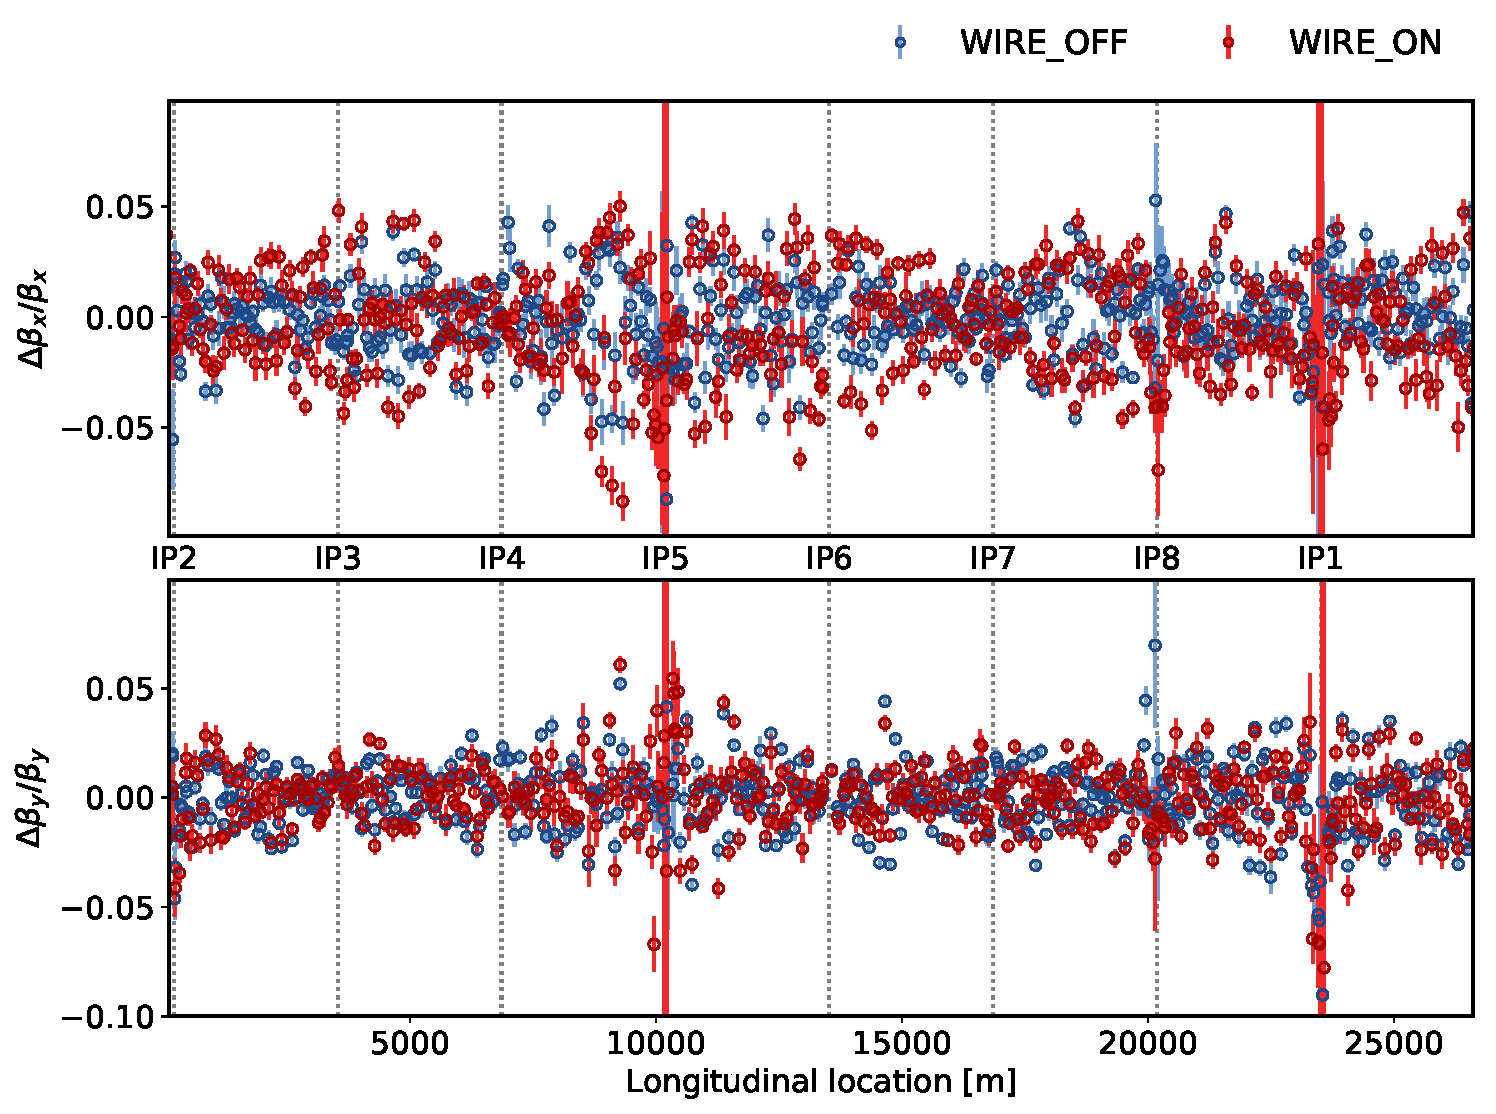
\includegraphics[width=.8\linewidth]{wire/beam1_beta_beat.pdf}  
  \caption{Beam~1}
\end{subfigure}
\begin{subfigure}{.5\textwidth}
  \centering
  % include second image
  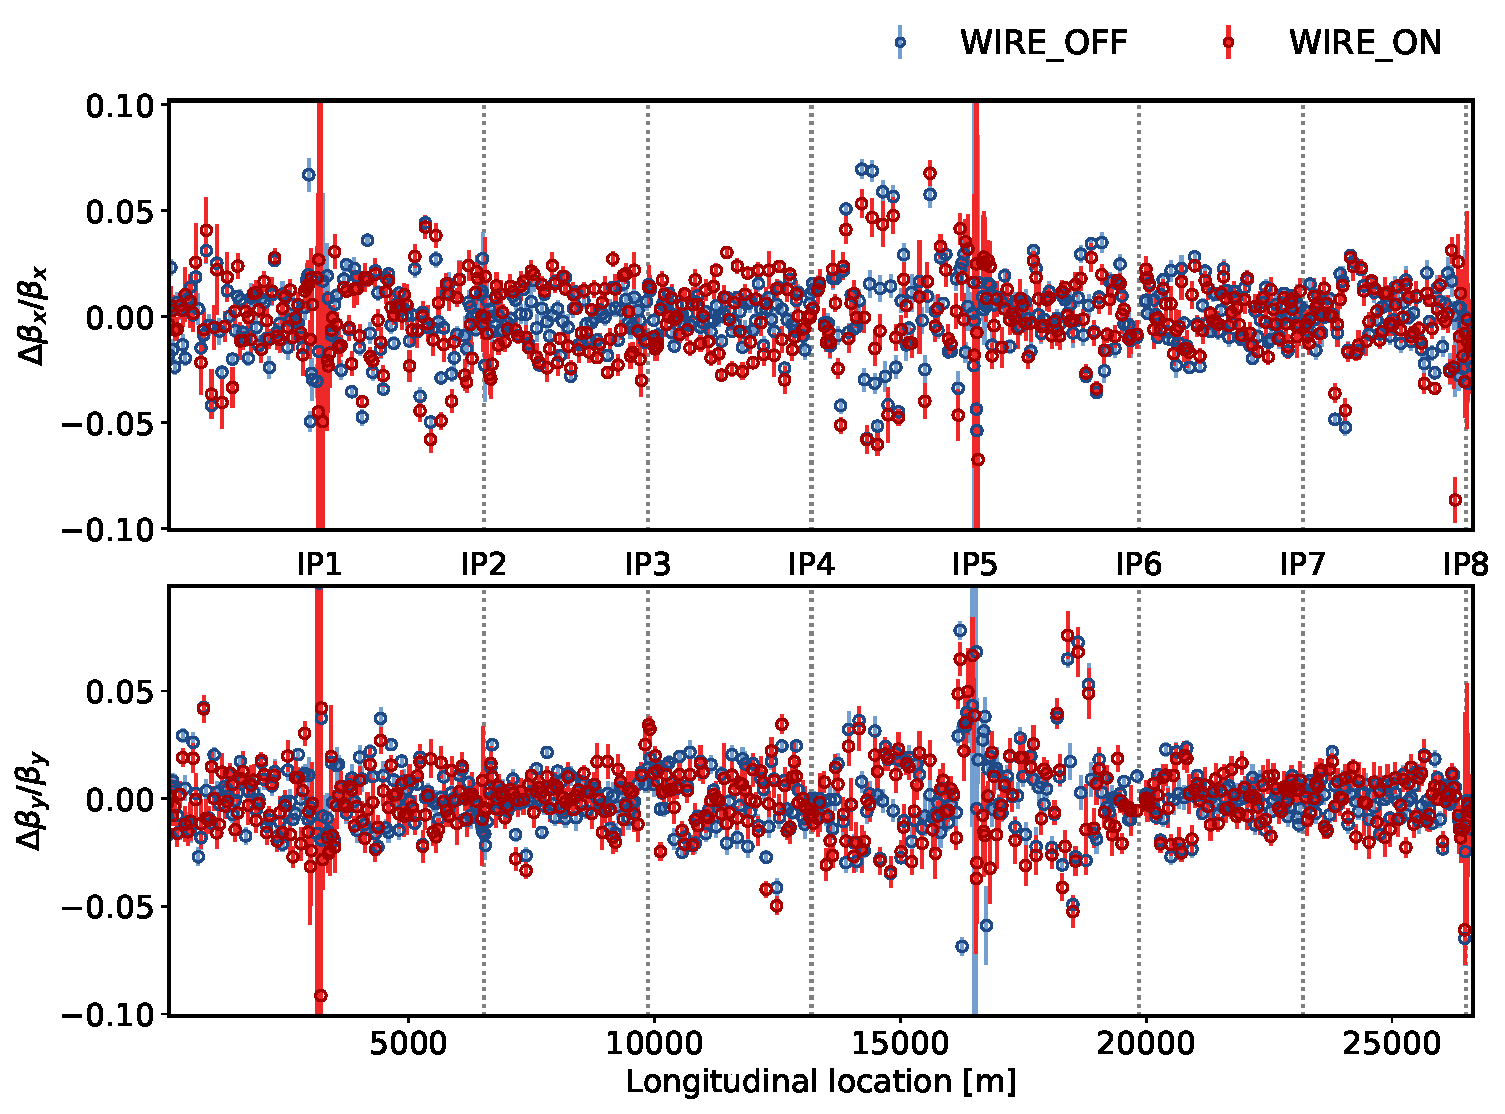
\includegraphics[width=.8\linewidth]{wire/beam2_beta_beat.pdf}  
  \caption{Beam~2}
\end{subfigure}
\caption{$\beta$-beat with the LRBB wire On and Off.}
\label{fig:before_after_pre_cycle}
\end{figure}


\bibliography{references}
\bibliographystyle{plain}

\end{document}